\chapter{Le développement du nouveau site}

Cette partie du rapport décrit le déroulement du développement du projet de façon chronologique, en commençant par l'analyse de nos besoins, en passant par l'élaboration d'une maquette jusqu'à l'implémentation de l'application.

\section{Réflexions préliminaires}

Lors de la première phase du projet, nous avons tout d'abord dû réfléchir aux besoins auxquels le site doit répondre.  
À travers plusieurs réunions hebdomadaires, nous avons alors réfléchi aux améliorations que nous souhaitions apporter par rapport à l’ancien site de l’\ofni\ et défini la liste des fonctionnalités que nous souhaitions implémenter.  

C'est également à ce moment-là que nous avons dû juger de la faisabilité de certaines fonctionnalités au regard du Règlement Général sur la Protection des Données (RGPD), qui régule et protège les droits des utilisateurs d'Internet dans l'Union Européenne.

\subsection{Les fonctionnalités du site}

Ainsi, après ces réunions, nous avons retenu plusieurs fonctionnalités principales pour répondre aux besoins de l'association et de ses membres. Le site comporte une page de présentation de l’association et de son histoire, ainsi qu’une page dédiée aux événements, permettant aux utilisateurs de s’inscrire et de gérer leurs inscriptions. Une page actualités permet de suivre les dernières informations concernant l’association.  

Une boutique en ligne a également été mise en place afin de permettre l’achat de produits ainsi que l’adhésion à l’association. Un espace galerie photo a été conçu pour partager les souvenirs des événements passés.  

En cours de projet, nous avons été amenés à ajouter une nouvelle fonctionnalité au site : un jeu ludique ayant pour objectif de donner envie aux étudiants de venir sur le site de façon régulière. L'idée nous a été proposée par un de nos tuteurs, Monsieur \propre{Demougin}, après la conception de la maquette. Cette idée nous a beaucoup plu, et nous avons alors décidé d'implémenter une version revisitée du célèbre jeu \logo{Space Invaders}: \game.
\pagebreak

Un formulaire de contact est mis à disposition des entreprises souhaitant entrer en relation avec l’association. Par ailleurs, une page administrateur a été intégrée pour faciliter la transmission et la gestion du site par les futurs bureaux de l’\ofni.  

Concernant les utilisateurs, un système de comptes a été mis en place. Un compte utilisateur permet d’accéder à la galerie photo, de jouer au jeu et de s’inscrire aux événements. De leur côté, les administrateurs disposent d’un compte spécifique leur permettant de gérer les événements, les actualités et les photos, ainsi que d’accéder aux paramètres avancés du site.

\subsection{Recherche sur les technologies}

Lors de ces réflexions, nous avons recherchés les technologies les plus adaptées pour développer un site performant et facilement maintenable par les futurs membres de l’association.
\bigskip

Afin de mieux gérer notre organisation, sur les conseils de nos tuteurs Monsieur \propre{Demougin} et Madame \propre{Pierrot}, nous avons adopté l’outil \logo{Trello}. Cet outil nous a permis de lister et d’organiser les différentes tâches à accomplir, tout en suivant leur état d'avancement. En collaboration avec nos tuteurs, nous avons ainsi identifié les fonctionnalités à implémenter et avons réparti leur développement au sein du groupe.
\bigskip

Pour le développement du serveur, nous avons choisi un framework \logo{PHP}, ayant déjà appris ce langage lors de l’unité d’enseignement \citer{Langages du Web} en deuxième année de licence. Ce choix nous permettait de nous concentrer sur l’architecture du projet sans devoir apprendre un nouveau langage, tout en assurant une continuité pour les futurs membres de l’association qui connaîtront également le \logo{PHP}, tant que ce langage reste au programme de licence du moins.
De plus, l'ancien site de l'\ofni\ étant hébergé sur un serveur \logo{PHP}, ce choix nous permettait de rester sur ce serveur et non de devoir souscrire à un autre.
\bigskip

Deux frameworks répondent à ces critères: \logo{Laravel} et \logo{Symfony}. Bien que ces deux outils partagent de nombreuses similarités, il existe d'un point de vue technique une différence fondamentale. Tandis que le premier utilise un paradigme de programmation dit \citer{fonctionnel}, le second est plutôt orienté objet. L'avantage de \logo{Laravel} est donc sa simplicité, tant pour la rédaction que pour son apprentissage, l'inconvénient est qu'il s'agit d'une approche que nous maîtrisons moins. Quant à \logo{Symfony}, la rédaction nécessite plus de travail mais la conception nous est plus naturelle étant donné que nous connaissons la programmation orientée objet depuis notre première année de licence.
\pagebreak

\section{Le maquettage du nouveau site}

Une fois ces réflexions achevées, nous avons entamé la conception de la maquette du site en deux étapes. Une première version manuscrite nous a permis de structurer le site de manière schématique, puis une version finalisée a été réalisée sur \logo{Figma}, un logiciel spécialisé dans la création de maquettes, afin d’obtenir un maquettage propre et exploitable.

L'objectif principal de cette maquette était de confirmer les fonctionnalités désirées et de commencer à visualiser leur implémentation et la forme qu'elles allaient prendre, sans se concentrer sur la charte graphique ni sur le design visuel du site.
\bigskip

Afin de travailler efficacement en groupe, nous avons réparti la charge de travail de manière équilibrée entre les membres de l'équipe. Pour la conception de la maquette, nous avons d'abord réfléchi ensemble aux différentes pages qui devaient composer le site, avant que chacun ne prenne en charge certaines d’entre elles. Cette répartition s’est faite naturellement, chacun ayant des préférences différentes.
\bigskip

Dans un premier temps, nous avons réalisé une esquisse manuscrite, tel que l'exemple de la \figureref{manuscrite} de la page de galerie photo, afin d’organiser les différentes pages du site et de positionner les éléments fonctionnels. Cette étape a été cruciale dans ce projet puisqu'elle nous a facilité la réflexion sur la structure générale du site et l'agencement des fonctionnalités.

C'est également ici que nous avons commencé à imaginer comment rendre notre site le plus maintenable possible sans ajouter de code supplémentaire. Nous avons pensé à créer la possibilité de gérer le contenu du site sans code (comme le ferait un Système de gestion de contenu comme \logo{Wordpress} par exemple)
Nous avons également imaginé et schématisé un système de génération de formulaires personnalisés pour les événements.

\begin{figure}[H]
    \centering
    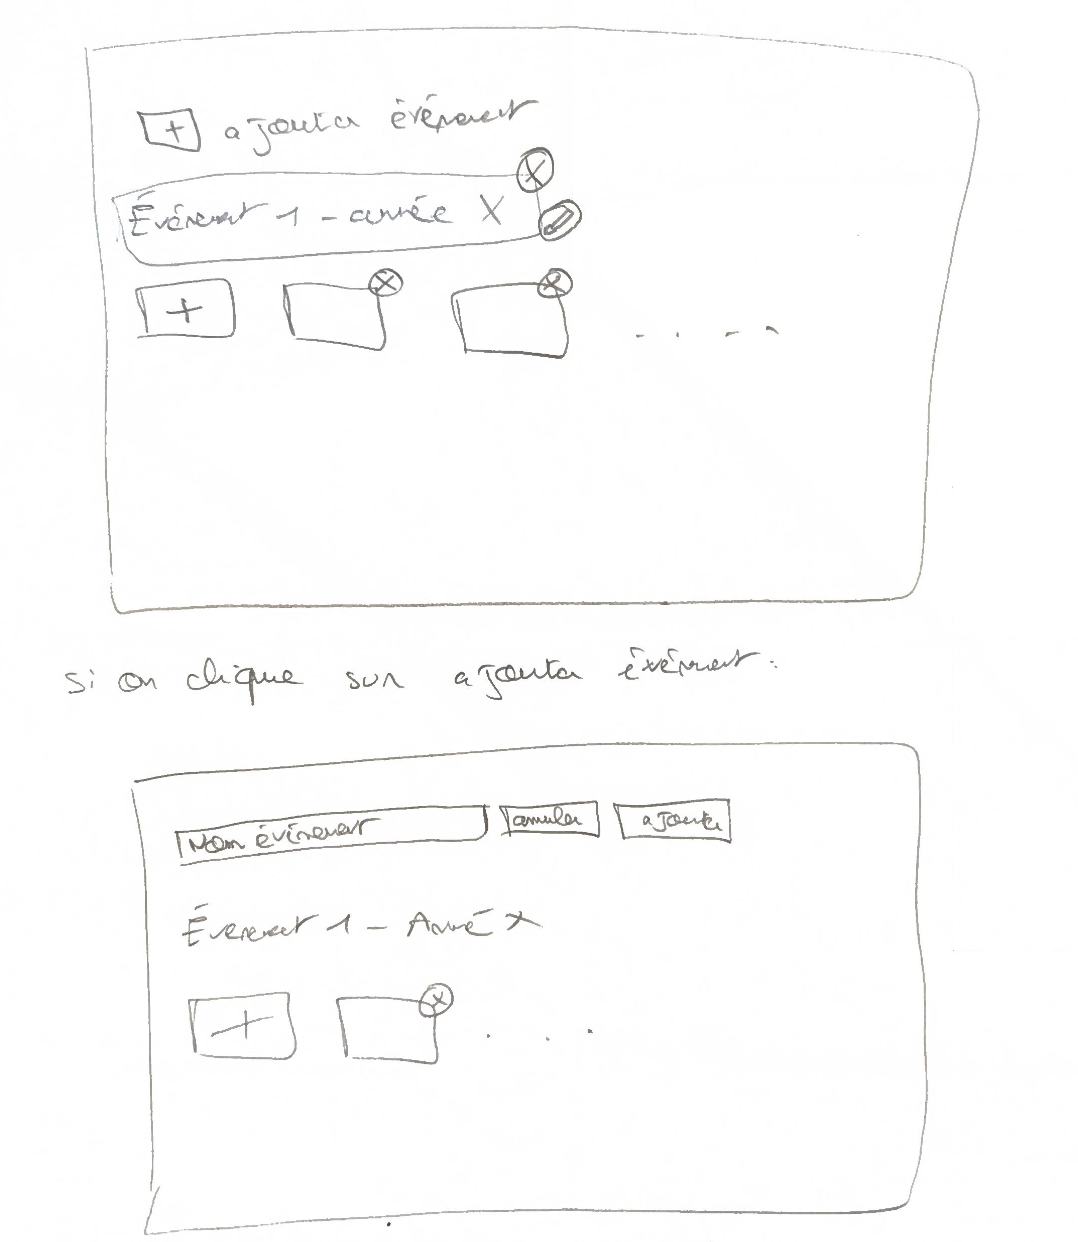
\includegraphics[width=10cm]{assets/pictures/maquette.png}
    \captionsetup{justification=centering}
    \caption{Page de la maquette manuscrite concernant la gestion de la gallerie photo}
    \label{manuscrite}%
\end{figure}
\bigskip

Une fois cette version manuscrite terminée, nous avons échangé avec nos tuteurs afin d’ajuster certains éléments.
Nous avons notamment été amenés à repenser la façon dont l'utilisateur devait interagir avec le site afin de rendre l'expérience la plus intuitive possible.

Après plusieurs ajustements, nous
avons commencé l'élaboration d'une version numérique finalisée sur l'outil \logo{Figma}, la \figureref{figma} montre un exemple de cette maquette.
Bien que nous ne connaissions pas le logiciel, nous avons pu rapidement le prendre en main et il nous a ainsi permis de transformer nos brouillons manuscrits en une maquette plus aboutie et fidèle à notre vision du projet.

De plus, l'apprentissage de \logo{Figma} nous a également permis de pouvoir effectuer des maquettes stylisées afin de trouver le visuel qu'on souhaitait appliquer au projet.
\bigskip

\begin{figure}[H]
    \centering
    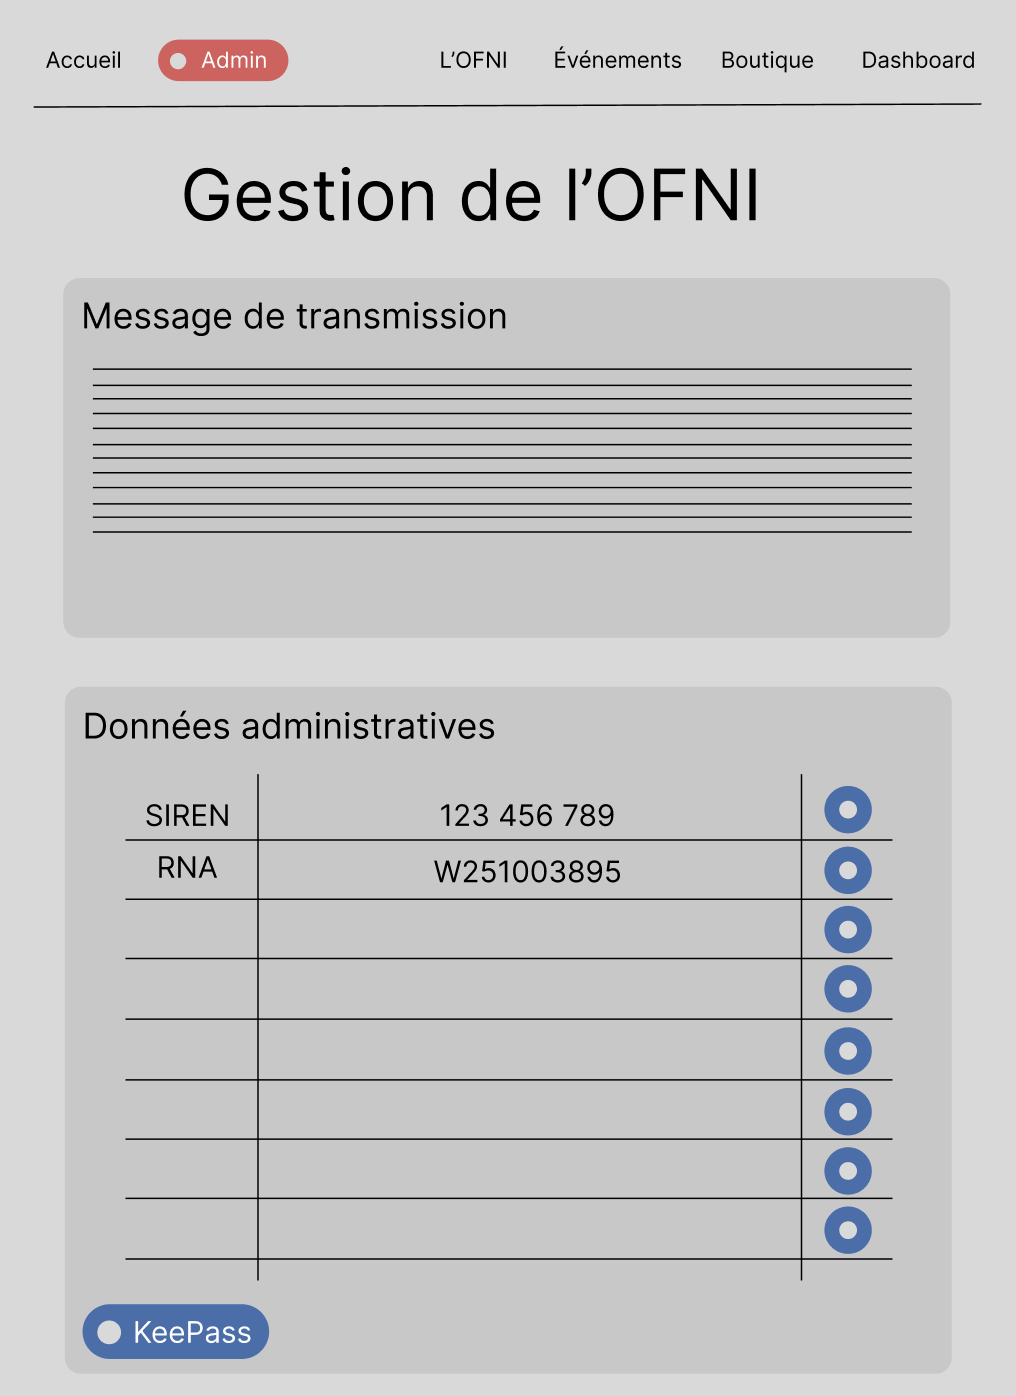
\includegraphics[width=10cm]{assets/pictures/figma.png}
    \caption{Page d'accueil de la maquette numérisée}
    \label{figma}
\end{figure}



\section{L'Implémentation du site}

Lors du développement du site, nous nous sommes accordés de sorte afin que chacun travaille de façon équitable et si possible sur ce qu'il apprécie faire le plus.
\bigskip

Concernant les technologies, nous avons décidé d'utiliser comme framework principal \logo{Symfony}. En effet, l'approche orientée objet sera plus facilement maintenable dans le futur puisque les étudiants qui reprendront l'association connaîtront bien ce paradigme. De plus, étant une technologie populaire en France, la présence d'une documentation en français ainsi que l'accès à beaucoup de ressources sur le sujet est un avantage pour cette dernière. Enfin, beaucoup d'entreprises françaises utilisent \logo{Symfony}, le connaître nous procure donc un avantage pour notre carrière professionnelle future.
\bigskip

Il convient alors de vous présenter brièvement comment \logo{Symfony} fonctionne.

Tout d'abord, tout code \logo{Symfony} est structuré en respectant l'architecture MVC, comme montré dans la \figureref{mvc}, ce qui signifie que chaque élément que l'on va ajouter à notre projet est divisé en trois parties : le \textbf{modèle} (M), la \textbf{vue} (V) et le \textbf{contrôleur} (C). 

Le \textbf{modèle} est la partie qui gère les données du projet. Il correspond aux entités et aux interactions avec la base de données. C’est grâce à lui que l’on peut stocker, récupérer et manipuler les informations essentielles au bon fonctionnement du site.

La \textbf{vue} est responsable de l'affichage des données et de l'interface utilisateur. Dans notre projet, nous avons utilisé \logo{Twig}, le moteur de \langue{template} de \logo{\logo{Symfony}}, afin de générer dynamiquement les pages \logo{HTML} en séparant la logique de la présentation.

Enfin, le \textbf{contrôleur} joue le rôle d’intermédiaire entre le modèle et la vue. Il reçoit les requêtes des utilisateurs, interagit avec le modèle pour récupérer ou modifier des données, puis choisit la vue à afficher en fonction du contexte. En \logo{\logo{Symfony}}, chaque contrôleur est une classe \logo{PHP} contenant des méthodes appelées "actions", qui déterminent la réponse renvoyée à l’utilisateur.

Grâce à cette architecture, le développement du site s’est fait de manière modulaire et organisée, facilitant ainsi l’ajout de nouvelles fonctionnalités et la maintenance du code sur le long terme.
\bigskip

\begin{figure}[H]
    \centering
    
\includegraphics[width=10cm]{assets/pictures/mvc.png}
    \caption{Architecture MVC dans Symfony}
    \label{mvc}
\end{figure}
\bigskip

Pour la conception de l'aspect visuel de nos pages web, nous avons décidé d'utiliser le préprocesseur \logo{Sass (Syntactically Awesome StyleSheets)}, dans l'objectif d’améliorer la structuration et la maintenabilité du code \logo{CSS}.

C'est un préprocesseur \logo{CSS} qui améliore et optimise l'écriture des styles en ajoutant des fonctionnalités avancées que \logo{CSS} natif ne propose pas.
L'objectif de ce préprocesseur est d'écrire du code \logo{Sass} qui sera ensuite compilé en \logo{CSS} pour être interprété par les navigateurs.

Il permet, entre autres, d’utiliser des variables, des imbrications de sélecteurs, des mixins (blocs réutilisables de styles), des fonctions et l’importation de fichiers, ce qui facilite l'organisation et la maintenabilité du code.
Grâce à \logo{Sass}, les fichiers \logo{CSS} peuvent être mieux structurés en étant divisés en plusieurs fichiers partiels (préfixés par '\logo{\_}'~), chacun correspondant à un élément spécifique du projet (variables, composants, mises en page, etc.). 
Ces fichiers sont ensuite importés dans un fichier principal, permettant ainsi une meilleure organisation et réutilisation du code.
\logo{Sass} utilise l’extension de fichier \logo{.scss}, qui reprend la syntaxe classique du \logo{CSS} tout en y ajoutant ces fonctionnalités avancées.

En automatisant certaines tâches et en limitant la redondance, Sass améliore la productivité des développeurs et rend le code plus lisible, évolutif et facile à maintenir sur le long terme.
\bigskip

Enfin, pour la réalisation du jeu, le langage JavaScript a été rapidement adopté, en raison de son intégration facile et de sa compatibilité avec la grande majorité des navigateurs.




\section{Les choix de développement}  
\label{sec:difficultes}

Plus concrètement, le maquettage du site se voit confrontée à plusieurs problématiques et interrogations, tant techniques qu'éthiques. Il est d'abord attendu de la structure du site une certaine factorisation. Puis, le stockage des données personnelles ainsi que la décision d'autoriser ou non une inscription, sont des questions qui sont à prendre en compte du début à la fin du développement.

\subsection{L'autorisation d'inscription}
\label{subsec:autorisation-inscription}

Pour s'inscrire aux événements de l'\ofni\, il est nécessaire de posséder un compte sur le site internet. La création d'un compte est réservée aux membres de l'\univ\~ ainsi qu'à certaines autres personnes, comme des alumni, sous réserve d'une autorisation manuelle du bureau de l'association.

Il faut alors trouver un élément concret qui permet de distinguer un membre de l'université d'une autre personne. Il est alors logique de se tourner vers les adresses e-mails. En effet, les adresses e-mails des membres de la faculté sont de la forme~: \code{prenom.nom@[edu.]univ-fcomte.fr}.

Lors de la réception d'une nouvelle demande d'inscription, l'algorithme doit donc simplement vérifier que l'adresse \langue{e-mail} de la personne soit conforme au spécimen précédent. Si c'est le cas, alors l'inscription est automatiquement validée à compter de l'instant ou la personne aura utilisé le lien de confirmation d'adresse qui lui a alors été envoyé. Sinon, il doit en faire manuellement la demande via le formulaire de contact situé sur la page d'accueil du site. Qu'importe la voie utilisée, une fois le compte créé, l'utilisateur peut alors s'inscrire aux différents événements.

\subsection{La génération de formulaire}
\label{subsec:generation-formulaire}

L'inscription à un événement nécessite, dans la quasi totalité des cas, le remplissage d'un formulaire par l'utilisateur. Ce dernier étant susceptible de changer à chaque événement, il est donc nécessaire de pouvoir générer dynamiquement ces formulaires en fonction des besoins. Pour cela, l'idée est alors de stocker les formulaires dans la base de données au format \logo{JSON}. Ainsi, lors de la création d'un événement, l'organisateur peut définir le formulaire qui doit être utilisé pour l'inscription. Si ce formulaire n'existe pas déjà, il peut alors le créer. Puis, lors de l'inscription, l'affichage du formulaire côté utilisateur est généré automatiquement en fonction des données stockées.

\subsection{La factorisation des événements}
\label{subsec:factorisation-evenements}

Avoir des formulaires réutilisables est un grand atout pour l'aspect \logo{CMS} du site. Mais au delà de l'inscription, la page utilisée pour présenter chaque événements, rique d'être très similaire d'année en année sur deux éditions d'un même événement. Il est alors nécessaire de pouvoir factoriser ces pages pour éviter de devoir tout recréer tous les texts et toutes les illustrations.
\bigskip

Pour pallier ce souci de factorisation, la structure du site permet alors à l'administrateur de créer d'abord un événement. Ce dernier est intemporel et n'est donc pas lié à une édition spécifique. Ce dernier centralise un nom, une illustration ainsi qu'un texte de présentation puis un autre texte de résumé. Dans un deuxième temps, l'administrateur peut alors créer une édition de cet événement. Cette édition est alors liée à l'événement et contient les informations spécifiques à son déroulement, comme la date, le lieu, le prix, etc. Ceci est, dans la terminologie du site, appelé une \citer{Instance d'événement}, faisant ainsi une petite référence au monde du développement, qui est après tout le point commun de tous les membres de l'\ofni.

Pour ce qui est de la page qui présente chaque édition d'un événement et fournit le lien d'inscription, elle est alors générée automatiquement à partir des données de l'instance d'événement.

